\chapter{Pruebas}


\begin{lstlisting}[language=cpp, 
				   caption={Pruebas lectura de valores potenciómetros},
				   label={lst:potenciometro_test_code}]
#include <Wire.h>
#include <LiquidCrystal_I2C.h>

#define MIN 0
#define MAX 100

LiquidCrystal_I2C lcd(0x27, 16, 2);
unsigned long  lastTimeUpdate=100;
int lastPulse;

void PotController(){
	int result, result2;
	int pot = analogRead(A0);
	int pot2 = analogRead(A1);
	result = map(pot, 0, 1024, MIN, MAX );
	result2 = map(pot2, 0, 1024, MIN, MAX );	
	lcd.clear();
	lcd.print(result); lcd.print("  "); lcd.print(result2);
}

void setup() {
	Serial.begin(9600);
	lcd.begin();
	lcd.backlight();
	lcd.print("RUN!");
}

void loop() {
	if (millis() > lastTimeUpdate) {
	PotController();
	lastTimeUpdate = millis() + 100;
	}
}
\end{lstlisting}




\begin{figure}[h]
\centering
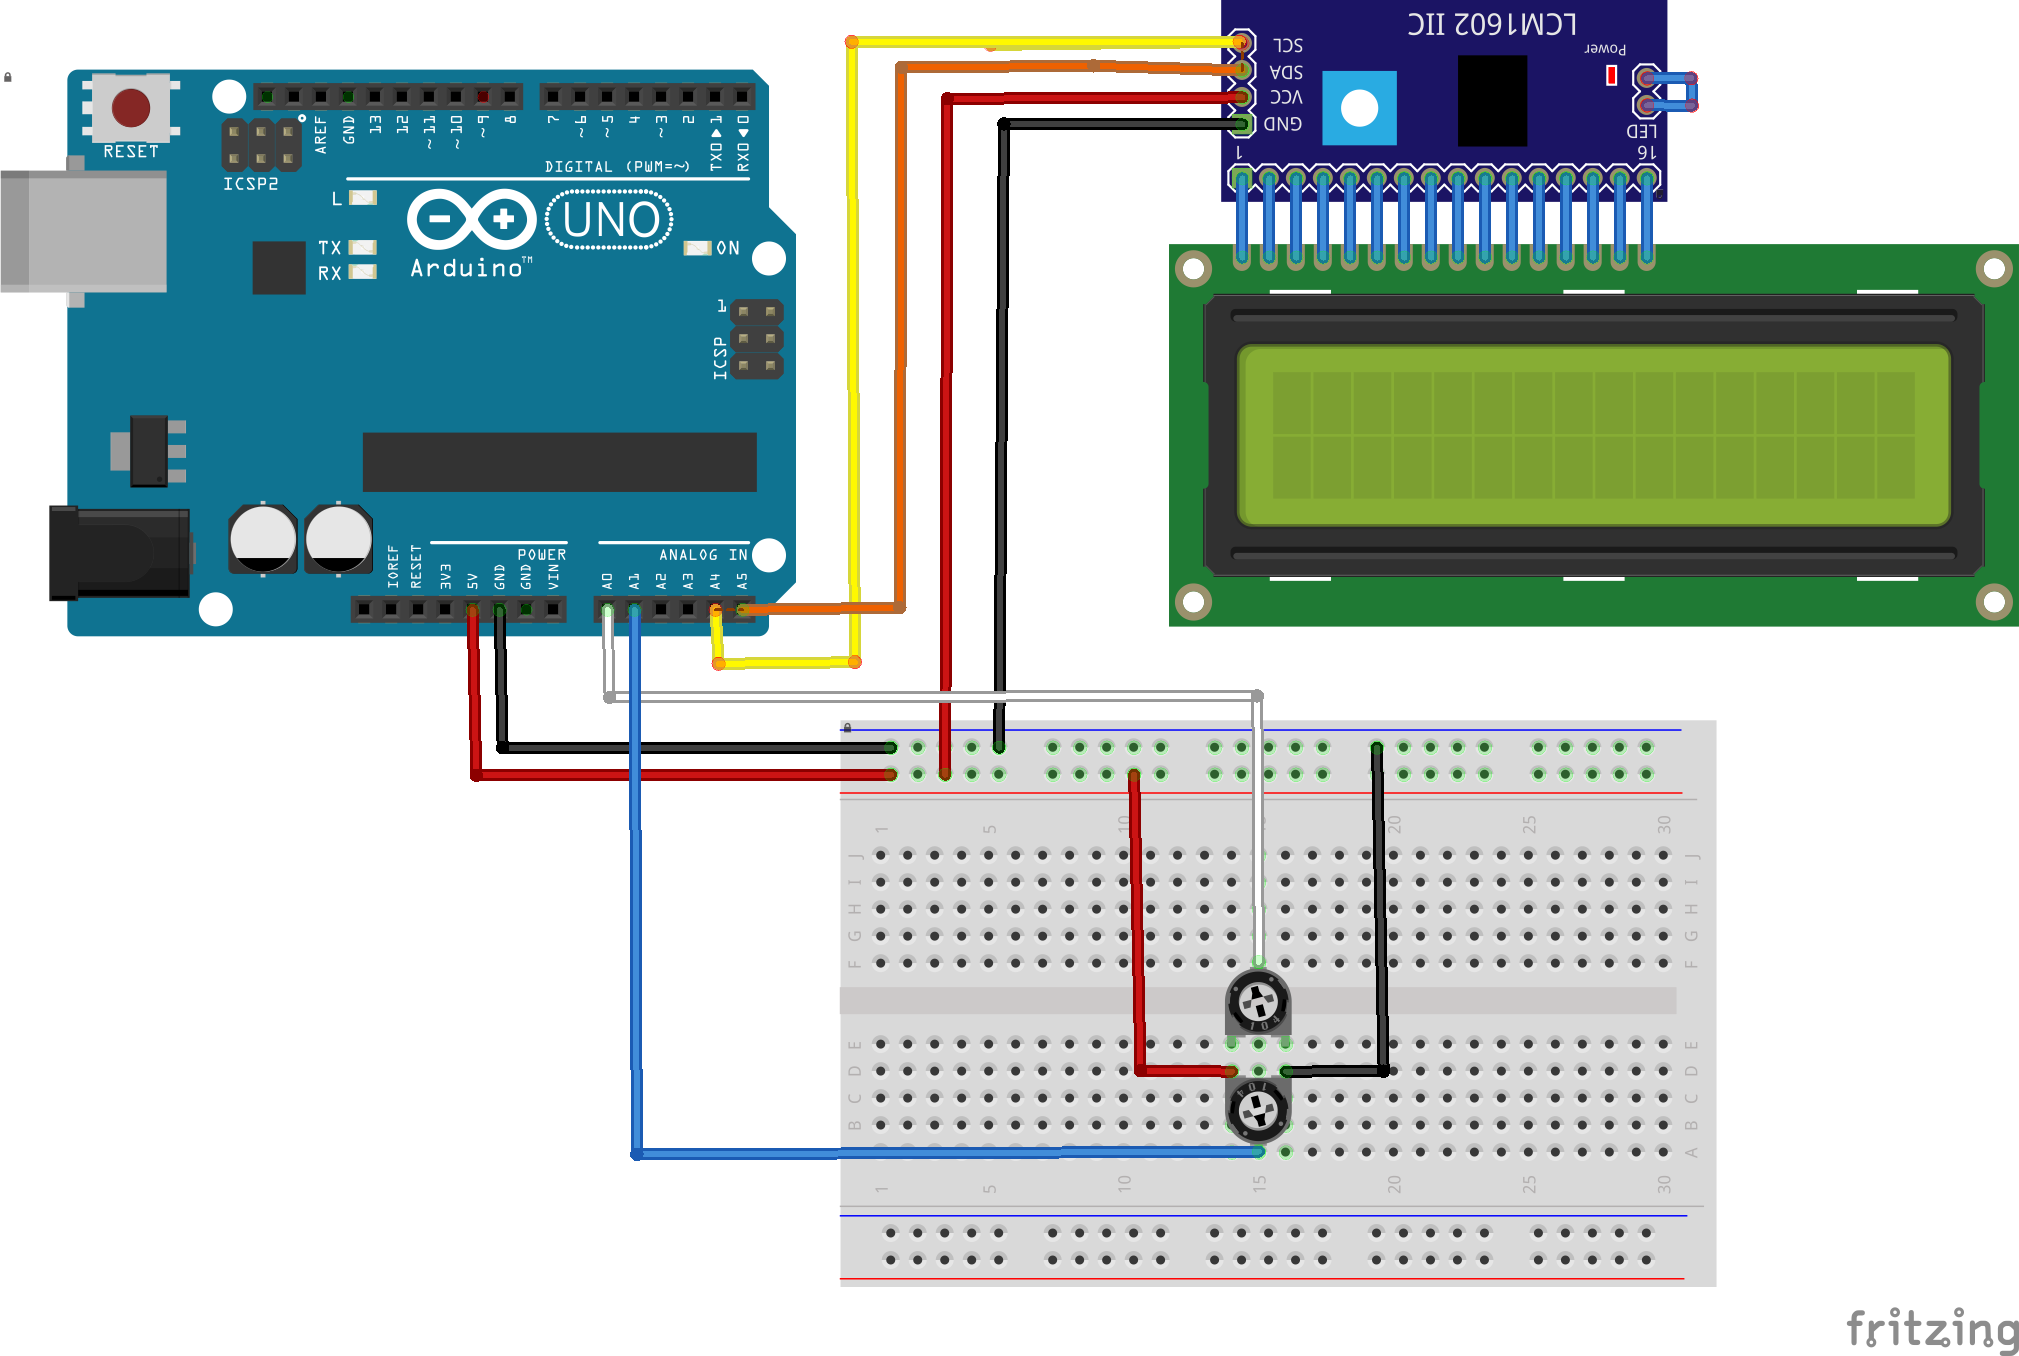
\includegraphics[width=0.9\linewidth]{../images/test_potenciometros}
\caption{Circuito para las pruebas lectura de valores potenciómetros}
\label{fig:test_potenciometros}
\end{figure}


\begin{lstlisting}[language=cpp,
				   caption={Prueba mover motor paso a paso},
				   label={lst:motor_test_code}]
#include <AccelStepper.h>
#define PINDIR 3
#define PINSTEP 2

AccelStepper motor(1, PINSTEP, PINDIR);

void setup() {
	Serial.begin(9600);
	motor.setMaxSpeed(500);
	motor.setAcceleration(100);
}

void loop() {
	motor.run();
	motor.moveTo(-3000);
}


\end{lstlisting}

\newpage

\begin{figure}[h]
	\centering
	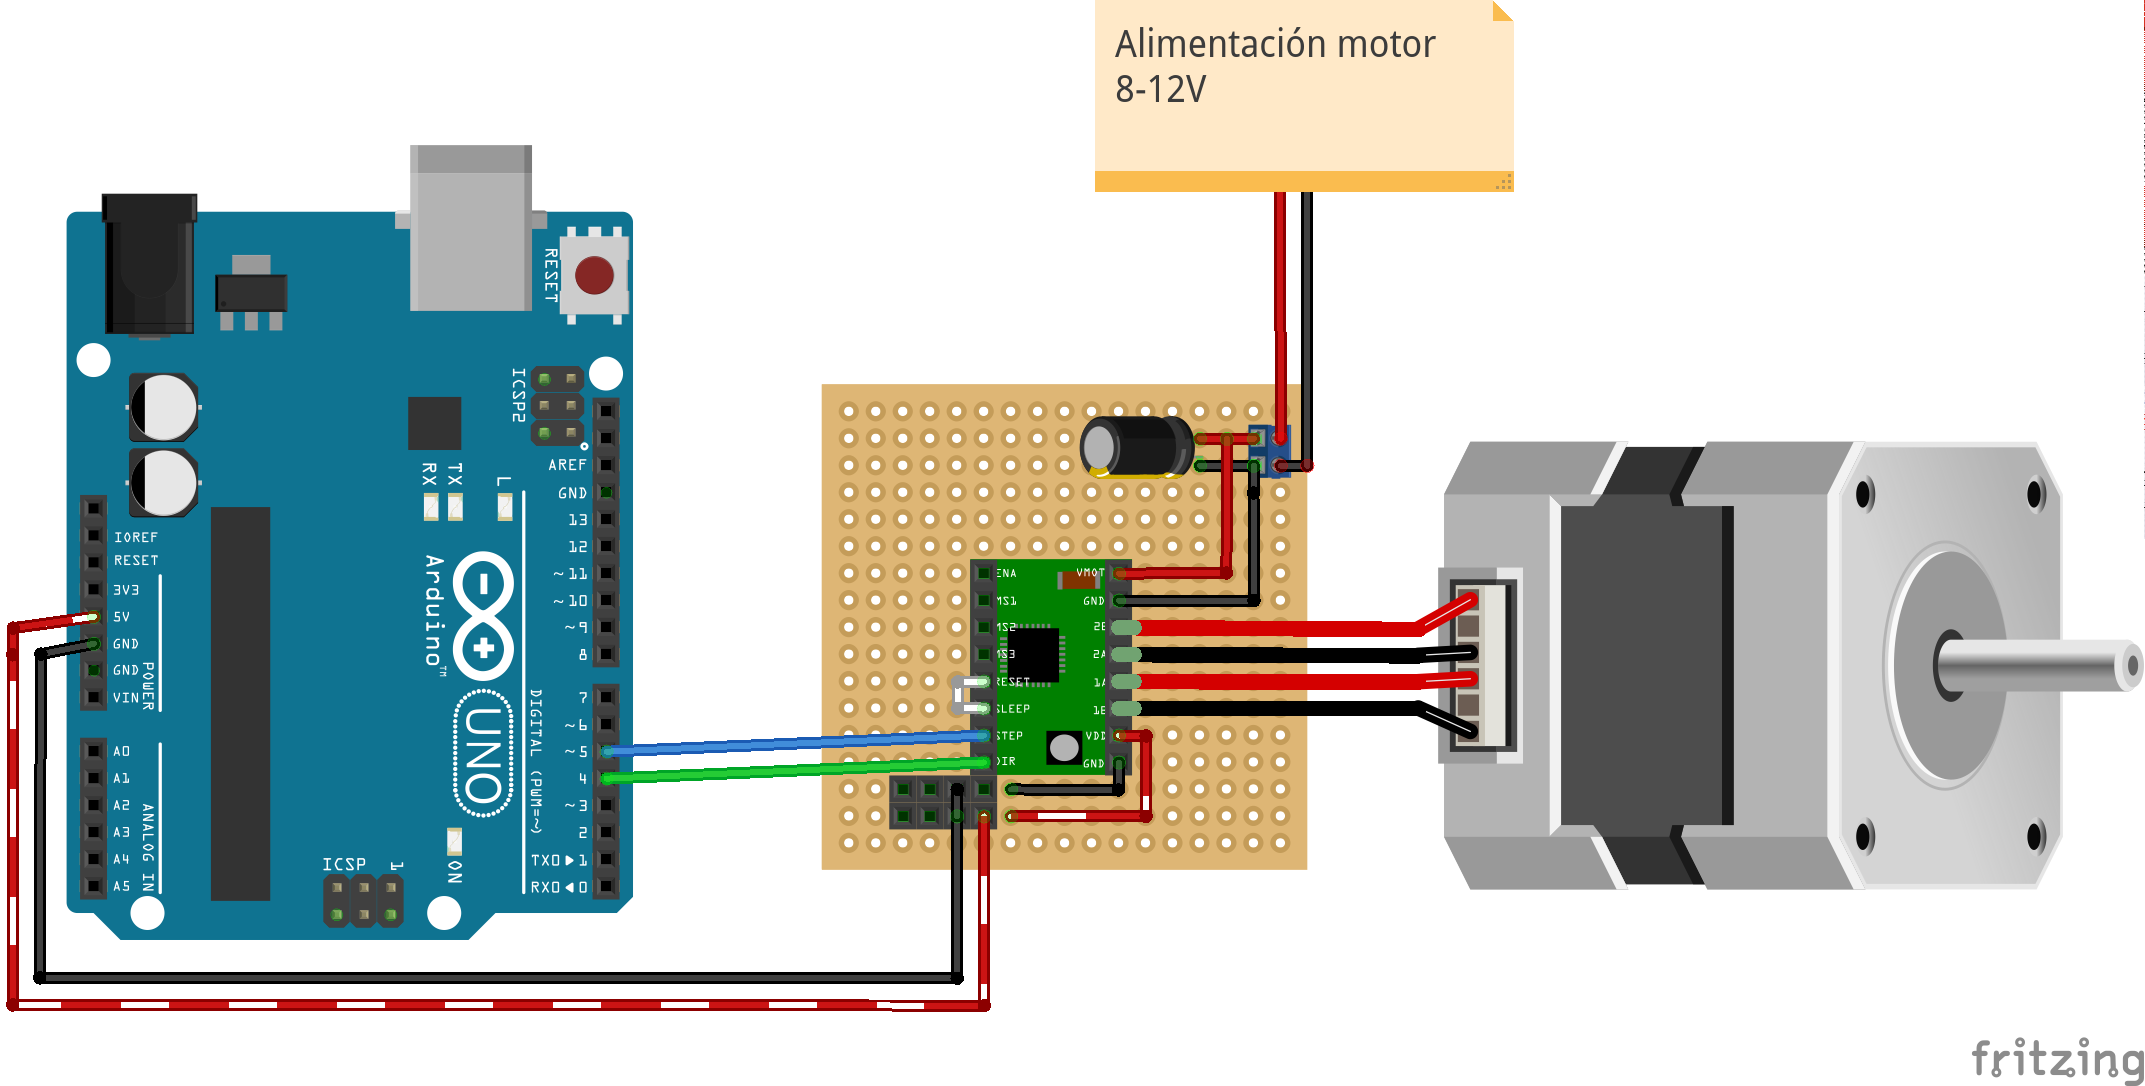
\includegraphics[width=0.9\linewidth]{../images/test_motor}
	\caption{Circuito para la prueba mover motor paso a paso}
	\label{fig:test_motor_circuit}
\end{figure}


\newpage
\begin{lstlisting}[language=cpp,
				   caption={Prueba Wii nunchuck},
				   label={lst:nunchuck_test_code}]
#include <Wire.h>
#include <math.h>
#include <nunchuck.h>
#include <LiquidCrystal_I2C.h>

LiquidCrystal_I2C lcd(0x27, 16, 2);
WiiChuck chuck = WiiChuck();
const int btnRIGHT=0, btnUP=1, btnDOWN=2, btnLEFT=3;
const int btnC=4, btnZ=5, btnNONE=6;
int lastTimeUpdate=1000;
int lastPulse;

void nunckuckController(){
	chuck.update();
	if(chuck.cPressed() && lastPulse!=btnC ){
		lcd.clear();
		lcd.print("C");
		lastPulse=btnC;
	}if(chuck.zPressed() && lastPulse!=btnZ){
		lcd.clear();
		lcd.print("Z");
		lastPulse=btnZ;
	}if(chuck.rightJoy() && lastPulse!=btnRIGHT){
		lcd.clear();
		lcd.print("RIGHT");
		lastPulse=btnRIGHT;
	}if(chuck.leftJoy()&& lastPulse!=btnLEFT){
		lcd.clear();
		lcd.print("LEFT");
		lastPulse=btnLEFT;
	}else  {
		lastPulse=btnNONE;
	}
}

void setup() {
	Serial.begin(9600);
	lastPulse=btnNONE;
	lcd.begin();
	lcd.backlight();
	chuck.begin();
	chuck.update();
}

void loop() {
	if (millis() > lastTimeUpdate) {
		nunckuckController();
		lastTimeUpdate = millis();
	}
}
\end{lstlisting}

\begin{figure}[h]
	\centering
	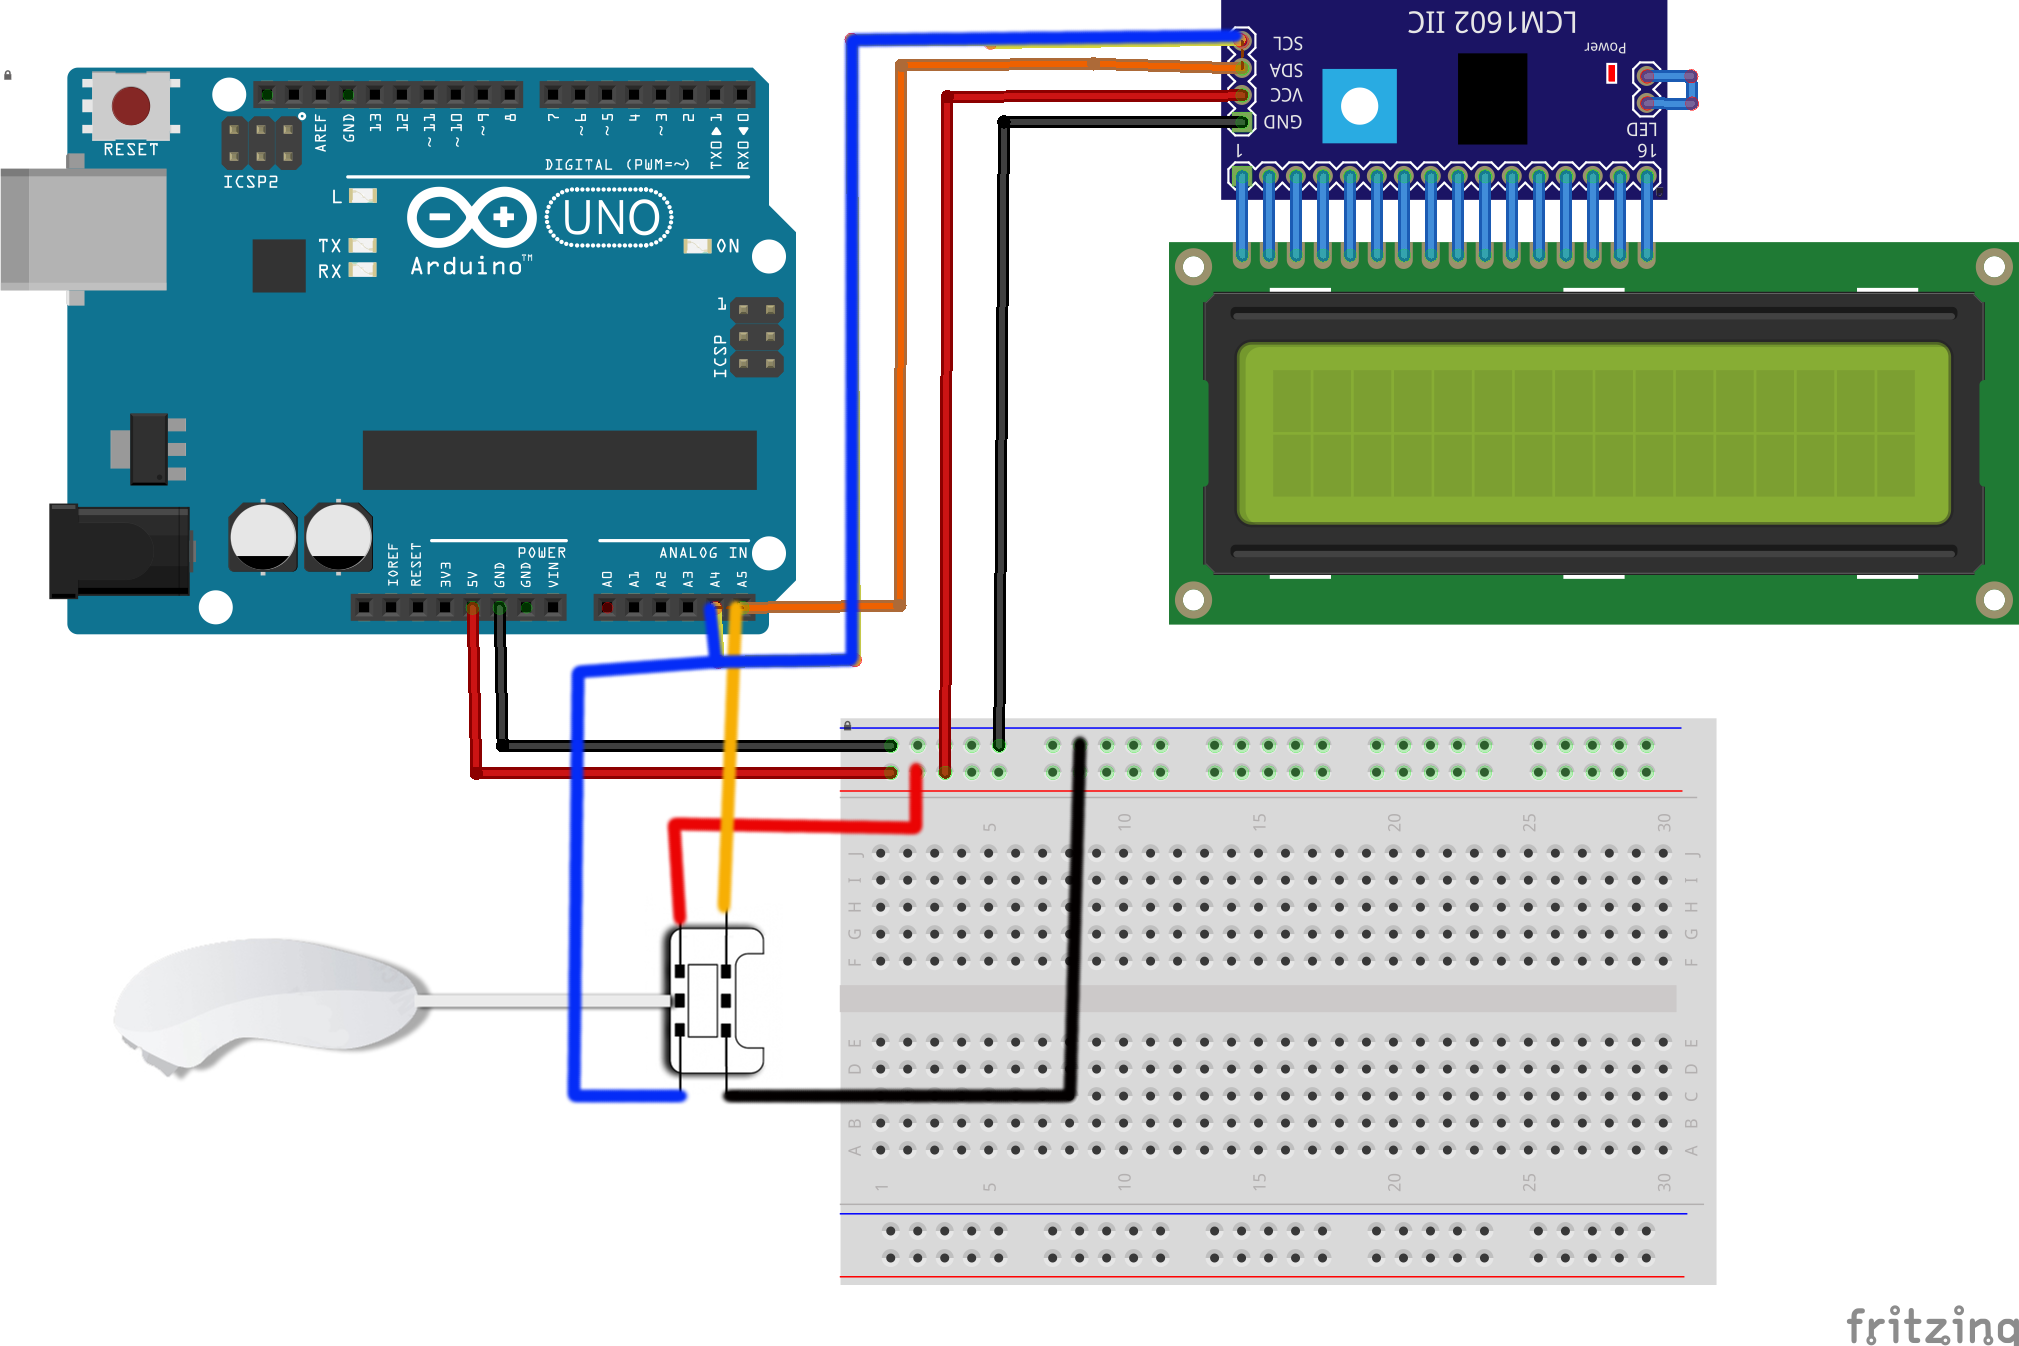
\includegraphics[width=0.9\linewidth]{../images/test_nunchuck}
	\caption{Circuito para la prueba Wii nunchuck}
	\label{fig:test_nunchuck_circuit}
\end{figure}







